\newpage
\section{Theorie}
\subsection{Elementare Strahler}
Es gibt zwei elementare Strahler. Der eine stellt eine E Feld Antenne dar, der andere eine H Feld Antenne. Die beiden elementaren Strahler lassen sich nicht praktisch fertigen, sie dienen nur für theoretische Überlegungen. 
\subsection{Hertzscher Dipol }
Ein elektrisch kurzer Linearstrahler kann als konzentriertes Bauelement betrachte werden. Auf seiner gesamten Länge kann ein Strom mit der komplexen Amplitude I und eine räumlich konstanten Stromverteilung, die zeitlich sinusförmig schwingt, annehmen. Es stellt sich einen kurzen Stromfaden ein, dessen Stromrichtung von der Polarisierung der Dipole abhängt und somit mit $\omega $ die Richtung wechselt. 
Der Hertzsche Dipol bildet den elementare Elektrischendipol, man kann ihn als sehr kurze Stabantenne vorstellen. Der Betrag des Dipolmoments \textit{p(t)} eines Hertzschendipos ist als \textit{p}=\textbf{Q}\textit{d}\textbf{\textbf{l}} beschrieben. Der Scheitelwert $\hat{i}$ des Stromes  oszilliert mit der Kreisfrequenz kleine omega $\omega$.\\
$p(t)=pe^{j\omega t} = Q dl e^{j\omega t} = \frac{\hat{i} dl}{j\omega }e^{j\omega t}  $
\\
Ist ein Hertzscher Dipol unendlich dünn und in einem xyz Koordinatensystem in die z Richtung ausgerichtet so gilt.
 
Es bildet sich ein E Feld von dem positiven Ladungspunkt zum negativen Ladungspunkt. Die Potentiale der Ladungspunkte oszillieren mit $\omega$. 
%\begin{center}
%\begin{minipage}{\linewidth}
%\centering
%\includegraphics{\conten\bilder\Herz_Dipol_EMANT_S37.pdf}%
%\captionof{figure}[kurze Bildunterschrift]{Bildunterschrift}%
%\end{minipage}
%\end{center}


\begin{figure}[!htb]
	\centering
	\includegraphics[width=4cm]{content/bilder/HerzDipolEMANTS37.pdf}%
	\caption{Hertzscher Dipol}
	\label{HerzDipol}
\end{figure}

%\begin{figure}[htbp]
%	\centering
%		\includegraphics[width=8cm]{content/Bilder/Z0_Grafik.png}
%	\caption{Wellenimpdedanz Z0}%
%	\label{Z0_Grafik}
%\end{figure}
Die Ausrichtung der E Feldlinien wechselt bei jeder Schwingung ihre Richtung. Im Nahfeld dominiert das E Feld. Mit wachsendem Abstand sind das E Feld und das H Feld senkrecht aufeinander und in Phase. Dabei können das E und H Feld als ebene Welle betrachtet werden. Die allgemeine Formel für die Feldverteilung laut:

Formel:
%E_r=(I dl)/2π  e^(-jkR) (n/R^2 +1/(jωεR^3 ))cos(θ)
%E_θ=(I dl)/4π  e^(-jkR) (jωμ/R+n/R^2 +1/(jωεR^3 ))sin(θ)
%H_φ=(I dl)/4π  e^(-jkR) (jk/R+n/R^2 )sin(θ)
\begin{equation}
E_r= \frac{I dl}{2\pi}   e^{-jkR} \left( \frac{n}{R^{2}}  + \frac{1}{j\omega \epsilon R^{3}}\right) cos(\theta)
\end{equation}

\begin{equation}
E_\theta= \frac{I dl}{4\pi}   e^{-jkR} \left( \frac{j\omega \mu}{R}  + \frac{n}{R^{2}}+ \frac{1}{j\omega \epsilon R^{3}}\right) sin(\theta)
\end{equation}

\begin{equation}
H_\phi= \frac{I dl}{4\pi}   e^{-jkR} \left( \frac{jk}{R}  + \frac{n}{R^{2}}\right) sin(\theta)
\end{equation}

Mit wachsendem Abstand können einige Terme vernachlässigt werden. Alle Terme in denen der Abstand R in höherer Potenz vorkommt werden vereinfacht zu Null. Für das Fernfeld ergeben sich die folgenden Beschreibungen:

Formel:
\begin{equation}
E_r= 0
\end{equation}

\begin{equation}
E_\theta= \frac{I dl}{4\pi}   e^{-jkR} \left( \frac{j\omega \mu}{R}  \right) sin(\theta)
\end{equation}

\begin{equation}
H_\phi= \frac{I dl}{4\pi}   e^{-jkR} \left( \frac{jk}{R} \right) sin(\theta)
\end{equation}

%Die Terme mit R in der zweiten oder dritten Potenz fallen für das Fernfeld weg. Da im Fernfeld der Radius R so gross ist, dass diese Terme vernachlässig werden. 
%Das Fernfeld kann wie folgt beschrieben werden:
%
%Formel:
%
%Die beiden elementaren Strahler können nicht technisch realisiert werden, aber sie sind sehr wichtig für das Verhalten von realen Antennen. Denn wenn reale Antennen verein-facht werden oder wenn sehr kleine Teilstücke von realen Antennen betrachtet werden, so verhalten sie sich oft wie die elementaren Dipole. 
%
%Die Dipolantenne und die Rahmen Antenne sind den beiden Elementaren Strahleren nachempfunden und sollen im nächsten Abschnitt genauer betrachtet werden.


\subsection{Fitzgeraldscher Dipol }
Eine unendlich dünne Leiterschleife die auf der ganzen Länge die selbe Stromverteilung besitz, wird Fitzgeraldscher Dipol genannt. Dieser Dipol ist das Gegenstück zum Hertzschen Dipol und stellt somit den zweiten der beiden elementaren Strahler dar. Die Leiterschleife ist oft in der xy Ebene angeordnet. Da der Strom oszilliert ist er als \textit{i(t)} gekennzeichnet. Der Strom \textit{i(t)} führt in einem Kreis im Abstand a um das Zentrum. Im Zentrum bildet sich ein magnetisches zeitabhängiges Moment \textit{m(t)}.
\begin{figure}[!htb]
	\centering
	\includegraphics[width=4cm]{content/bilder/Fitzgerald_Dipol_EMANT_S37.pdf}%
	\caption{Fitzgeraldscher Dipol}
	\label{FitzDipol}
\end{figure}
Wenn der Hertzsche Dipol eine E Feld Antenne genannt wird, so ist der Fitzgeraldsche Dipol eine H Feld Antenne. Das Nahfeld des Fitzgeraldschen Dipols wird wie folgt beschrieben:
Formel:
%H_r=IS/2π  e^(-jkR) (jk/R^2 +1/R^3 )cos(θ)
%H_θ=IS/4π  e^(-jkR) (-k^2/R+jk/R^2 +1/R^3 )sin(θ)
%E_φ=nIS/4π  e^(-jkR) (k^2/R-jk/R^2 )sin(θ)
\begin{equation}
H_r= \frac{I S}{2\pi}   e^{-jkR} \left( \frac{jk}{R^{2}}  + \frac{1}{R^{3}} \right) cos(\theta)
\end{equation}

\begin{equation}
H_\theta= \frac{I S}{4\pi}   e^{-jkR} \left(- \frac{k^{2}}{R}  + \frac{jk}{R^{2}}+ \frac{1}{R^{3}} \right) sin(\theta)
\end{equation}

\begin{equation}
E_\phi= \frac{I S}{4\pi}   e^{-jkR} \left( \frac{k^{2}}{R}  - \frac{jk}{R^{2}} \right) sin(\theta)
\end{equation}

Die Terme mit R in der zweiten oder dritten Potenz fallen für das Fernfeld weg. Da im Fernfeld der Radius R so gross ist, dass diese Terme vernachlässig werden. 
Das Fernfeld kann wie folgt beschrieben werden:

Formel:
\begin{equation}
H_r= 0
\end{equation}

\begin{equation}
H_\theta= \frac{I S}{4\pi}   e^{-jkR} \left(- \frac{k^{2}}{R}   \right) sin(\theta)
\end{equation}

\begin{equation}
E_\phi= \frac{I S}{4\pi}   e^{-jkR} \left( \frac{k^{2}}{R}   \right) sin(\theta)
\end{equation}

Die beiden elementaren Strahler können nicht technisch realisiert werden, aber sie sind sehr wichtig für das Verhalten von realen Antennen. Denn wenn reale Antennen verein-facht werden oder wenn sehr kleine Teilstücke von realen Antennen betrachtet werden, so verhalten sie sich oft wie die elementaren Dipole. \\

Die Dipolantenne und die Rahmen Antenne sind den beiden Elementaren Strahleren nachempfunden und sollen im nächsten Abschnitt genauer betrachtet werden.

\subsection{Die Dipol Antenne}
Der zentral gespeist Dipol besteht meist aus runden Leiterstäben mit dem Durchmesser d die ananeinander liegen so, dass in der Mitte der beiden Stäbe eine kleine Lücke entsteht. Die gesamte Länge der beiden Stäbe entspricht 2l>>d. Wird eine Spannung wird in der Lücke zwischen den beiden Stäbe angelegt, kommt es zu einer Stromverteilung über die Länge der beiden Stäbe. Oft wird die Spannung mit einer 2 Draht Leitung,  diese wird auch Transmission Line genannt, zwischen den Leiterstäben angebracht. Die anschliessende Stromverteilung der beiden runden Leiterstäbe liefert der Ursprung der Wellenausbreitung. In erster Näherung kann die sich vom der Speisestelle ausbreitende Wellenausbreitung als richtugnsunabhänige Kugelwelle betrachtete werden.
%E^j(wt-kr)/4pimu^-1 r
%Elliot Seite 29 Nr1.93
\begin{equation}
\frac{e^{j(\omega t-kr)}}{4\pi \mu_{0}^{-1}r}
\end{equation}

\begin{figure}[!htb]
	\centering
	\includegraphics[width=4cm]{content/bilder/Dipol_EMANT_S42.pdf}%
	\caption{Dipol Antenne mit Stromverteilung}
	\label{FitzDipol}
\end{figure}

Die Stromausbreitung in deiner Dipol Stabantenne entspricht der Stromverteilung einer am Ende offenen Zweidrahtleitung. Das offene Ende der Leitung führt zur einer Reflexion der zuführenden Welle in die umgekehrte Richtung und somit zu einer stehenden Welle. Stromführende Elemente die nahe beieinander liegen, der Amplituden gleich aber gegenläufig sind, strahlen nur gering, das sind genau die Eigenschaften einer guten Zweidrahtleitung.
Als Näherung für die Stromverteilung soll folgendes gelten:
\begin{equation}
I(x,t) =I_{m}sin([k(l-x)])e^{j\omega t}
\end{equation}
%Elliot Seite 59 Formel 2.1

Bei einem Dipol mit dem Durchmesser $d<<\lambda$ wird der Dipol zu einem dünnen Stromfaden und der Leiter kann \textbf{J}\textit{d}\textbf{\textbf{J}} mit \textbf{I}\textit{d}\textbf{\textbf{l}} als Stromelement ersetzen. Die Summation der Elementardipole kann dann als Quelle betrachtet werden.\\

\begin{equation}
I_{m}sin(k(l-dz))
\end{equation}
%Elliot Seite 61 Formel 2.2
Die Gewichtungsfunktion dieser Summe von Elementardipolen die alle in der z Achse liegen ist:\\
$a(\phi)= 0$
aber die Gewichtungsfunktion in $\theta$ Richtung:
\begin{equation}
a_{\theta}(\theta)=- \frac{2I_{m}}{k sin(\theta)} \lbrack cos(kl cos(\theta)) - cos(kl) \rbrack
\end{equation}
%Elliot Formel 2.6 oder Joss EMANT 122.

Es sollen zwei Fälle genauer betrachtet werden.
\begin{itemize}
\item der Halbwellendipol mit 2l= $\lambda/2$
\item der kurze Dipol mit 2l<<$\lambda$
\end{itemize}
\subsubsection{lambda/2 Dipol  Halbwellendipol}
Der $\lambda/2$ Dipol ist eine der wichtigsten Antennen. Über die Gewichtungsfunktion lässt sich auf das Fernfeldverhalten schliessen.
\begin{equation}
E_{\theta}=j60I_{m} \frac{e^{j(\omega t - kr)}}{r} \lbrack \frac{cos\lbrack  (\pi/2) cos(\theta)\rbrack}{sin(\theta)} \rbrack
\end{equation}
\begin{equation}
H_{\phi}=j \frac{I_{m}}{2\pi} \frac{e^{j(\omega t - kr)}}{r} \lbrack \frac{cos\lbrack  (\pi/2) cos(\theta)\rbrack}{sin(\theta)} \rbrack
\end{equation}
%E(theta)= Ellito 2.8
%E(phi) = Ellito 2.9

Die Feldverteilung kann in der 2 Dimensionalen Polar Form oder in einer 3 Dimensio-nalen Feldverteilung dargestellt werden.
Die nachfolgende Grafik zeigt eine E Feldverteilung als Schnitt durch die xz Ebene.\\
Bild aus Mtlab importiern\\
\begin{figure}
\begin{center}
\begin{tikzpicture}
	\draw (0,3) -- (10,3);%Fadenkreuz horizontal
	\draw (5,0) -- (5,6);%Fadenkreuz vertikal
	\draw [line width=1mm] (5,3.2) -- (5,4.5);%upper arm
	\draw [line width=1mm] (5,1.5) -- (5,2.8);%lower arm
	\draw (3,3) circle (2cm);%linker Kreis
	\draw (7,3) circle (2cm);%rechter Kreis

	\node[draw] at (5,6.5) {$\theta=0$};
	\node[draw] at (8,5.5) {$E(\theta)$};
\end{tikzpicture}
\end{center}
	\caption{Dipol Antenne E Feld}
	\label{DipolEFerd}
\end{figure}
Dargestellt ist ein $\lambda/2$ Dipol der in z Richtung aufgerichtet ist. Es ist zu erkennen, dass bei $\theta = 0 ^\circ $  und $\theta = 180 ^\circ $ kein elektrisches Feld abgestrahlt wird. Stellt man sich die Grafik als um eine um phi von 0 Grad bis 360 Grad rotierende Scheibe vor, so kommt die bekannte Doughnut Form zum Vorschein.

Die von theta und phi abhängige Leitung ist gegeben durch:
%P(theta,phi)= elliot2.10
\begin{equation}
P(\theta,\phi)=\frac{2\eta I_{m}^{2}}{(4\pi r)^{2}}\lbrack \frac{cos^{2}\lbrack (\pi/2) cos(\theta)\rbrack}{sin^{2}(\theta)}\rbrack
\end{equation}

%Durch Lösung des Doppelintegrals 
%Elliot Seite 63
Durch auflösen der Doppelintegrale über $\phi$ von 0 bis $\pi$  und $\theta$ von 0 bis $\pi$ Erhält man eine nummerische Lösung der Integrale über die gesammte Kugelfäche aufintegriet von: 
\begin{equation}
P_{rad}=0.609 \frac{\eta I_{m}^{2}}{2\pi}
\end{equation}
%elliot 63 Forlmel 2.11

Wie die obere Grafik ganz gut zeitgt ist die maximale Feldausbreitung auf höhe der Einspeisestelle bei $\theta = 90 ^\circ $, denn der  $sin(90 ^\circ ) =1$ entspricht.
Der maximale Richtwert  aus dem englischen als directivity bekannt erhält man indem die Abgestrahlte Leitung mit einem isotropen Kugelstrahler verglichen wird.
\begin{equation}
D(peak)=\frac{P(\theta,\phi)(\pi/2)}{P_{rad}/ 4 \pi r^{2}} =1.64
\label{eq:Directivity}
\end{equation}
%Dmax=1.64 nach Ellito 2.12

Bei $l=\lambda/4 $ ist der Scheitwert des Antennenstromes, beim Einspeisepunkt, dem Zentrum des Dipol bei z= 0, bei $I_{m}$. Somit kann gesagt werden, dass die Zuleitung  die folgende Leitung  liefert:
%Elliot 2.14
\begin{equation}
P=\frac{1}{2} I_{m}^{2}R_{rad}=(0.609)\frac{\eta I_{m}^{2}}{2\pi}
\end{equation}

Der Strahlungswiderstand oder auch $R_{rad}$ genannt kann im Fall des $\lambda /2$ Dipol nummerisch als 73 Ohm bestimmt werden.
\begin{equation}
R_{rad}=\frac{0.609 \eta}{\pi}= 73 Ohm
\end{equation}
\subsubsection{Der kurze Dipol mit 2l<<Lambda}
Die Therme $cos(kl*cos(\theta)) $ und $cos(kl)$ aus der Gewichtungsform des $\lambda/2$ Dipol können mit einer Reihe angenähert werden sofern kl klein ist.
\begin{equation}
a_{\theta}(\theta)=-kl^{2}I_{m}sin(\theta) \lbrack 1- \frac{(kl)^{2}}{12}(1+cos^{2}(\theta))+...\rbrack
\end{equation}
%Ellito 2.15 Seite 64
Der Eingangsstrom eines kurzen Dipol ist gegeben durch:
\begin{equation}
I=I_{m}sin(kl)=I_{m}\lbrack kl - \frac{(kl)^{3}}{3!} +... \rbrack
\end{equation}
%Ellito 2.16
Sogar für kleine Längen wie 2l = $\lambda/4 $ kann ohne grossen Fehler die Gewichtingsfunktion als 
%Ellito 2.17
\begin{equation}
a_{\theta}(\theta)=-kl^{2}I_{m}sin(\theta)=-Ilsin\theta
\end{equation}
angenommen werden.
Wie beim $\lambda/2$ Dipol findet man bei einem kurzen Dipol ein vertikal polarisiertetes E Feld. Das Feld ist etwas breiter aber ebenfalls doughnutförmig. Die Impedanz des kurzen Dipol ändert sich jedoch drastisch gegenüber dem Lambda/2 Dipol. Und mit der Impdanz ist auch die winkelabhänige Leistungsdichte wie folgt gegeben:
%Ellito 2.18
\begin{equation}
P(\theta,\phi)=\frac{(kl)^{2}\eta I^{2}}{2(4\pi r)^{2}}sin^{2}\theta
\end{equation}
Die abgestrahlte Leitung eines kurzen Dipol bei dem über die ganze Kugeloberfläche mit dem Radius r integriert wurd kann mit
%Ellito 2.19
\begin{equation}
R_{rad}=20(\frac{\pi L}{\lambda})^{2}
\end{equation}
berechnet werden.\\

Die aus der abgestrahlten Leitung ergebenden maximale Richtwirkung eines kurzen Dipol wird  mit einem isotopen Strahler verglichen und es ergibt nach Formel \ref{eq:Directivity} einen Wert für D=1.5. Das ist nicht viel weniger als bei einem $\lambda/2$ Dipol mit einem D Wert von 1.64.
Der Strahlungswiderstand kann mit der Umformung des $Prad=1/2 I^{2}Rrad$ umgestellt werden. \\
Man findet :
$Rrad=20\left(piL/\lambda\right)^{2}$
%Eliott

Dabei wird L als 2l und somit als länge der beiden Dipolarme angenommen.
Wenn ein Dipol sehr kurz wird, zum Beispiel $2l=\lambda/8$ dann wird $R_{rad} = 3 Ohm$, dieser Wert ist merklich kleiner als die 73 Ohm die für einen Lambda/2 Dipol gefunden wurden. Der Effekt auf den reaktiven Anteil der Eingangsimpedanz ist noch dramatischer. Für einen endlich dünnen Dipol mit der Dicke d , ist die Reaktanz der Ein-gangsimpedanz eines $2l=\lambda/2$ positiv. Die Reaktanz ist wenig unter Null wenn die $2l=\lambda/2$ sind, aber wird der Dipol weiter gekürzt, so sinkt die Reaktanz sehr schnell immer mehr negativ. Im Fall, dass $2l=\lambda/8$ ist, so sind Werte für X grösser als 1000 Ohm kapazitive keine Seltenheit. 

\subsection{Loop Antenne}

\begin{figure}[!htb]
	\centering
	\includegraphics[width=7cm]{content/bilder/Loop_EMANT_S45.pdf}%
	\caption{Loop Antenne}
	\label{LoopAntenne}
\end{figure}
Wird eine kurze, kreisförmige, Stromschleife mit dem Radius $a<<\lambda$ von einem Strom $Ie^{j\omega t}$ durchflossen, dann kann in guter Näherung einen konstante Stromverteilung I entlang der Schlaufe angenommen werden,
Die Koordinaten eines Punktes auf der Stromschleife sind gegeben mit
\begin{eqnarray}
x’ &=&a \cos(\psi)\\
y’ &=&a \sin(\psi)\\
z’ &=&0
\end{eqnarray}


A ist der Abstand vom Zentrum der Stromsschleife. Somit kann ein Stromelement auf der Schleife beschrieben werden
\begin{equation}
I dl= Ia(- \vec e_{x}sin(\psi)+\vec e_{y}cos(\psi))d\psi
\end{equation}
 
%EMANT Joss Seit 45
Die Stromverteilung führt zu einem Abstrahlen von Elektromagnetischen Wellen.
%Die Gewichtungsfaktoren findet man mit Hilfe von (116 Joss) und (117 Joss) zu
%Emant Joss Seite 46
%Emant Joss Seite 46
Da eine Integration über $2\pi $ einer Kreisfunktion Null ergibt, findet man direkt 
\begin{equation}
a(\theta, \phi) =0
\end{equation}

Nimmt man zudem an, dass ka klein ist, so kann der folgende Therm verwinfacht werden sin(ka $sin(\theta)$cos($\psi$))=ka sin($\theta$)cos($\psi$) so findet man 
\begin{equation}
a(\theta)=j(\pi a^{2}I)(k sin \theta)
\end{equation}
%$a(theta, phi)=j$... oder Ellito 2.31 oder Joss Seite 46.
Das Fernfeld ist somit horizontal polarisiert (es ist phi polarisiert) und die Leistungsdichte gewinnt man mit 
%(Joss 118) 
\begin{equation}
\vec P(\theta,\phi)=\frac{1}{2}Re(\vec E x \vec H^*)
\end{equation}
zu
%Joss EMANT P(theta,phi)=....Ellito 2.32
\begin{equation}
P(\theta)=\frac{(ka)^{4}I{2}\eta}{32r^{2}}sin^{2}\theta
\end{equation}
Im Vergleich mit dem kurzen Dipol erzeugt die kleine Stromschleife ein vergleichbares Richtdiagramm. Das Fernfeld des kurzen Dipols ist jedoch vertikal(theta) polarisiert. Das bedeutet, dass die Abstrahlverhalten um 90Grad unterschiedlich sind. Integriert man die Leistungsdichte über eine Kugeloberfläche mit dem Radius r  auf uns setzt sie der abgegebenen Leistung mit $1/2 I^{2}Rrad $ der zugeführten Zweidrahtleitung gleich, so gewinnt man $R_{rad}$ mit 
\begin{equation}
R_{rad} = 320\pi^{6} (a/\lambda)^{4}
\end{equation}
%ELLITOH 2.33
Als Beispiel, wenn $a/\lambda = 0.003$ ist, dann wird der $R_{rad} = 0.25 Ohm$. Als Vergleich mit dem kurzen Dipol mit der Länge $2l=\lambda= 0.06$ führt das zu einem Strahlungswiderstand $R_{rad}$ von 0.7 Ohm.  Der Abstrahlwiderstand Rrad einer kleinen Stromschleife kann um den Faktor $n^{2}$ erhöht werden, wenn n die Anzahl der sehr eng aneinanderliegenden Wicklungen der Stromschleife sind. 




\begin{figure}
\begin{center}
\begin{tikzpicture}
	\draw (0,3) -- (10,3);%Fadenkreuz horizontal
	\draw (5,0) -- (5,6);%Fadenkreuz vertikal
	\draw (3,3) circle (2cm);%linker Kreis
	\draw (7,3) circle (2cm);%rechter Kreis
	\draw (4.5,3) circle (0.2cm);%linker kleiner Kreis
	\draw (5.5,3) circle (0.2cm);%rechter kleiner Kreis
	\draw (4.5,3.2) -- (5.5,3.2);%Verbindung horizontal oben
	\draw (4.5,2.8) -- (5.5,2.8);%Verbinung horizontal unten
	\node[draw] at (5,6.5) {$\theta=0$};
	\node[draw] at (8,5.5) {$E_{\phi}(\theta)$};
\end{tikzpicture}
\end{center}
\caption{Loop Antenne E Feld}
\label{DipolEFerd}
\end{figure}
\subsection{Systemanasicht}
Die Systemanasicht soll einen Überblick über die Bluetooth Verbindung vom Fluginstrument „Connect 1“ zu einem Smartphone geben.
In der nachfolgenden Tabelle werden die Annahmen und fest gegebenen Parameter der Bluetooth Verbindung aufgelistet. Mit der Hilfe des Linkbudgets kann eine Abschätzung des Antennengewinn auf der Empfängerseite hergeleitet werden. Um diese Abschätzung möglich zu machen, werden einige Annahmen getroffen. Zum Beispiel geht man von einer optimalen Anpassung der HF Quelle zur Antenne aus. Weiter wird der Luftraum zischen Sender und Empfänger als Vakuum angenommen und es hat keine Fremdkörper im Ausbreitungsraum.
Weitere Annahmen sind:
\begin{itemize}
\item Als Sende und Empfangschip wird beim Empfänger und Sender der CC2541 von TI eingesetzt
\item 	Freiraum ist Vakuum
\item Keine Hindernisse auf der Übermittlungsstrecke
\item Reserve von 6 dB

\item Der Gewinn der Sendeantenne ist 1
\item Die Sendeleistung ist 0 dBm
\item Die Anschluss und Verbindungsdämpfung beim Sender und beim Empfänger entsprechen je 0.5 dB
\item -94 dBm Empfangsempfindlichkeit bei 1Mbps und 0.1\% EBR des CC2541 von TI
\end{itemize}
\subsubsection{Linkbudget}
Tabelle
\subsection{Speisung}
Unter der Speisung der Antenne wird die Leistungszufühung verstanden. Damit eine Antenne strahl, muss diese mit einer Spannungswelle angeregt werden. Die Strom und Spannungsverteilung der Antenne ist für das Abstrahlverhalten verantwortlich. 
\subsubsection{Quelle}
Jedes Antennensystem verfügt über eine Quelle.  Die Quelle liefert an ihrem Ausgang ein Hochfrequentes Signal. Der Ausgang kann entweder symmetrisch oder asymmetrisch sein. Die Ausgangsimpedanz der Quellen kann sehr unterschiedlich sein. Oft findet sich am Quellenausgang ein Anpassnetzwerke um die Quellenimpedanz an die Leitungsimpedanz anzupassen.
\subsubsection{Zuleitung}
Darunter versteht man die Verbindung zwischen Quelle und Antenne. Je nach System kommen Zweidrahtleitungen, Koaxialkabelleitungen oder Hohlleiter zum Einsatz. Eine Zweidrahtleitung ist eine symmetrische Verbindung, während ein Koaxialkabel eine asymmetrische Verbindung darstellt.
\subsubsection{Anpassung}
Die Anpassung oder auch Impedanzanpassung genannt, kommt immer dann zum Zuge, wenn auf einem Signalpfad Stossstellen auftreten. Stossstellen treten immer dann auf wenn die Impedanz eines Leitermediums oder ein Übergang eines Bauteil ansteht. 
Man vergleicht immer die Eingangsimpedanz mit der Ausgangsimpedanz. Es ist also von Zein und Zaus die rede.
Es gibt zwei Arten von Anpassung.
\begin{itemize}
\item 	Leisungsanpassung
\item 	Singalanpassung
\end{itemize}
Leistungsanpassung wird benötigt, wenn der Leistungsfuss möglichst unbeeinträchtigt sein soll. Es muss gelten
Zein=Zaus*
Das bedeutete, dass der Realanteil von Zein und Zaus gleich ist aber der Imaginäranteil von Zaus muss den konjugiertkomplexen Wert des Zein aufweisen. Mit anderen Worten, Zaus hat beim Imaginärenanteil ein umgekehrtes Vorzeichen als der Zein. Leistungsanpassung kommt bei Leistungsendstufen oder allgemein dort zur Anwendung wo es besonders wichtig ist, dass möglichst viel der erzeugten Leistung von der Last aufgenommen wird. Man bedenke, das ist im besten Fall nie mehr als 50%.
Siganlanpassung wird angewendet, wenn möglichst keine Reflexionen auf der Leitung entstehen sollen. Es muss gelten:\\
Zein= Zaus\\
Die Siganlanpassung ist dann gewünscht, wenn die Qualität des Signals Vorrang hat, wenn keinerlei Reflexionen erwünscht sind. In diesem Fall ist das Stehendewellenverhältnis SWR = 1.
Um die jeweilig gewünschte Anpassung zu erreichen kommen Anpassnetzwerke zum Einsatz. Diese sind meist passive Netzwerke mit Induktivitäten L und Kapazitäten C, manchmal kommen zu den L und C ein Widerstand R hinzu.\\
Ein Beispiel für Anpassung\\
Eine Quelle mit einem Ausgangssiderstand von nicht 50 Ohm reell. Wird mit Hilfe eines ersten Anpassnetzwerk auf eine 50 Ohm Leitung angepasst. Am Ende der 50 Ohm Leitung wird ein weiteres Anpassnetzwerke benötigt, um die Leitung und die Antennen aufeinander abzustimmen.\\
\begin{figure}[!htb]
	\centering
	\includegraphics[width=8cm]{content/bilder/Anpassung.pdf}%
	\caption{Blockschaltbildeiner Anpassung von der Quelle zur Antenne}
	\label{Anpassung}
\end{figure}
Wenn eine 50 Ohm Leitung an eine Antenne angeschlossen wird, dann wird oft eine Anpassnetzwerk zischen der Leitung und der Antenne benötigt. Das Ersatzschaltbild einer Antenne zeigt weshalb. Antennen haben deben dem reelen Strahlungswiderstnad $R_{rad}$ je nach Typ einen kapazitiven oder induktiven Anteil. Wird das wie im nachfolgenden Bild nicht berücksichtigt, kommt es zu Reflexionen am Ende der Leitung.\\
\begin{figure}[!htb]
	\centering
	\includegraphics[width=5cm]{content/bilder/ESB_Antenne.pdf}%
	\caption{Ersatzschaltbild einer Antenne}
	\label{ESBantenne}
\end{figure}

\begin{figure}
	\begin{center}
	\begin{tikzpicture}
	\draw[line width=1.5pt](3, 3.5) circle (0.5) node at (3,3.5) {Uq};
	\draw[line width=1.5pt] (3, 5) -- (4.5, 5);
	%\draw[line width=1.5pt] (3, 2) -- (7, 2);
	\draw[line width=1.5pt, -o](3, 2)  -- (7, 2);
	\draw[line width=1.5pt] (3, 2) -- (3, 3);
	\draw[line width=1.5pt] (3, 4) -- (3, 5);
	\draw[line width=1.5pt](4.5, 4.75) rectangle (5.5, 5.25) node at (5, 5.5) {Rq} node at (5, 4.5) {50 Ohm};
	%\draw[line width=1.5pt] (5.5, 5) -- (7, 5);
	\draw[line width=1.5pt, -o](5.5, 5)  -- (7, 5);
	
	\draw[line width=1.5pt](7, 1.5) rectangle (12, 5.5) node at (9.5, 6) {Anpassungsnetzwerk};
	\draw[line width=1.5pt, o-](12, 5)  -- (13.5, 5);
	\draw[line width=1.5pt, o-](12, 2)  -- (16, 2);
	\draw[line width=1.5pt](13.5, 4.75) rectangle (14.5, 5.25) node at (14, 5.5) {Rv};
	\draw[line width=1.5pt](14.5, 5)  -- (16, 5);
	\draw[line width=1.5pt](16, 5)  -- (16, 4.4);
	\draw[line width=1.5pt](15.75, 3.4) rectangle (16.25, 4.4) node at (17, 3.9) {Rrad};%Rrad
	\draw[line width=1.5pt](16, 3.4)  -- (16, 2.8);
	\draw[line width=1.5pt](15.75, 2.8)  -- (16.25, 2.8);%Kondensator oben
	\draw[line width=1.5pt](15.75, 2.6)  -- (16.25, 2.6);%Kondensator unten
	\draw node at (17, 2.7) {Xant}
	\draw[line width=1.5pt](16, 2.6)  -- (16, 2);
	
	\draw[line width=1.5pt, ->, >=latex](6.5, 4)  -- (8, 4) node at (8, 3.5) {Pein};
	\draw[line width=1.5pt, ->, >=latex](11.5, 4)  -- (13, 4) node at (13, 3.5) {Pant};
	
	\coordinate (A) at (7, 1);
	\coordinate (B) at (7, 0);
	\coordinate (a) at (10, 0.5);
	\draw[line width=1.5pt, cap=round,->](A) .. controls (a) .. (B) node at (6.5, 0.5) {S11};
	\end{tikzpicture}
	\end{center}
\caption{Quelle}
\label{Quellel}
\end{figure}


\section{Design}
\subsection{Anforderungen}
Das Design des Antennensystem wird für einen Anwendungsfall im Freiraum dimensioniert. Die Distanz zwischen Sender und Empfänger soll 10 Meter betragen. Das Übertragungsmedium ist Luft kann aber idealisiert als Vakuum angenommen werden. Das System soll isotrop abstrahlen und der Gewinn der Empfangsantenne kann mit einem Faktor  1 angenommen werden. Die Antenne soll symmetrisch gespiesen werden und im 2.4 GHz ISM Band arbeiten. Als Quelle dient ein Bluetooth Low Energie Texas Instruments CC2541 Chip mit 0dBm als Sendeleistung. Als Designkriterien wird eine S11 Dämpfung von 10 dB und eine Reserve von 6 dB dienen.
\\
%\subsection{Technische Spezifikationen und Anforderungsliste}
%%\todo{Anforderungskatalogs mit Fest-, Mindest- \& Wunschforderungen}
%\begin{itemize}
%\item Geräte Connect 1
%\item Materialien des Gehäuse ABS Kusnstoff
%\item Volumen des Antennensystems
%\item Wirkungsradius 10m im Freiraum
%\item Richtcharakteristik isotroph
%\item Polarisation linear
%\item Antennen Wirkungsgrad ist zubestimmen
%\item Antennen Gewinn gleich wir der Abstrahl Wirkungsgrad
%\item minimaler Empfangspegel am Transceivers
%\item Transceivers Baustein Texas Instruments CC2541
%\item Sendeleistung
%\item $S_{11} \leq$ 10 dB
%\end{itemize}
\begin{tabular}{l|c|c|c|c}
\hline 
Nr. & Anforderung & Beschreibung & Wert & nicht erfüllt \\ 
\hline 
\hline 
001 & f & ISM Frequenzbereich  & 2.4-2.5 GHz & \\ 
\hline 
002 & f & Handgerät lxbxh & lxbxh &   \\ 
\hline 
003 & f & symmetische Speisung des Antennensystems &  \\ 
\hline 
004 & f & Reflexionskoeffizient der Antenne S11 & 10dB & \\ 
\hline 
005 & f & Funkdistanz, Arbeitsradius & 10m &  \\ 
\hline 
006 & f & Linkbudget Reserve & 6dB &  \\ 
\hline 
%• &  &  &  &  \\ 
%\hline 
%• &  &  &  &  \\
%\hline 
%• &  &  &  &  \\ 
%\hline 
%• &  &  &  &  \\ 
%\hline 
%• &  &  &  &  \\ 
%\hline
%• &  &  &  &  \\ 
%\hline 
%• &  &  &  &  \\
%\hline 
\end{tabular} 

\begin{figure}
\begin{center}
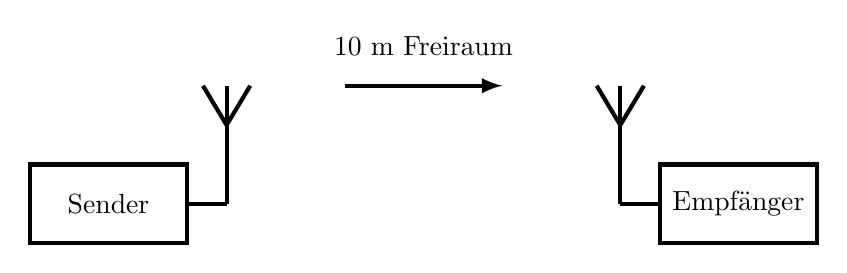
\begin{tikzpicture}
	\draw[line width=1.5pt](0, 0) rectangle (2, 1) node[pos=0.5] {Sender};
	\draw[line width=1.5pt] (2, 0.5) -- (2.5, 0.5);
	\draw[line width=1.5pt] (2.5, 0.5) -- (2.5, 1.5);
	\draw[line width=1.5pt] (2.5, 1.5) -- (2.2, 2);
	\draw[line width=1.5pt] (2.5, 1.5) -- (2.8, 2);
	\draw[line width=1.5pt] (2.5, 1.5) -- (2.5, 2);
	
	\draw[line width=1.5pt, ->, >=latex](4, 2)  -- (6, 2) node at (5, 2.5) {10 m Freiraum};
	
	\draw[line width=1.5pt] (7.5, 0.5) -- (8, 0.5);
	\draw[line width=1.5pt] (7.5, 0.5) -- (7.5, 1.5);
	\draw[line width=1.5pt] (7.5, 1.5) -- (7.2, 2);
	\draw[line width=1.5pt] (7.5, 1.5) -- (7.8, 2);
	\draw[line width=1.5pt] (7.5, 1.5) -- (7.5, 2);
%	\draw[line width=1.5pt,decorate,decoration=expanding waves](3, 2) -- (5, 2);
	\draw[line width=1.5pt](8, 0) rectangle (10, 1) node[pos=0.5] {Empfänger};
	%\node[draw,text] at (1,0.5) {Sender};
%	\node[draw,text] at (9,0.5) {Empfenger};
\end{tikzpicture}
\end{center}
\caption{Verbindungs Model}
\label{LinkModel}
\end{figure}

\subsection{Analyse mit bekannten Modellen}
\subsection{Neue Design Ansätze}